\documentclass[addpoints,12pt]{exam}
%\documentclass[12pt]{article}
\usepackage[letterpaper, margin=0.75in]{geometry}
\usepackage{graphicx}
\usepackage{enumitem}
\usepackage{booktabs}
\usepackage{tabularx}
\usepackage{amsmath}
\usepackage{color}

\begin{document}
\footer{}{Page \thepage\ of \numpages}{}

\begin{center}
\includegraphics[width=10cm]{../images/logo.png}
\end{center}

\begin{center}
\noindent{\LARGE Conceptual Physics \\ Answers to Questions from Homework Packet 3\\}
\end{center}

\noindent This document tries to answer the following questions:
\begin{enumerate}
	\item How does water evaporate when gravity pulls it down?
	\item Do planets and moons have electrical charges? If so, why wouldn't they attract each other and collide?
	\item How does high tide relate to the full moon?
\end{enumerate}

\clearpage

\section{Water Evaporation and Gravity}

\noindent\textbf{Question:} How does water evaporate when gravity pulls it down?

\noindent The short answer is that water molecules on the surface of the water gain enough energy from the thermal fluctuations of the surrounding molecules to break free of the liquid and become a gas. These molecules have much more kinetic energy, and are able to rise despite gravity trying to pull them back down, up to a limit -- once they reach a high enough altitude all of their kinetic energy is turned into gravitational potential and they stop rising. This is why, although gasses (such as water molecules, oxygen, nitrogen, carbon dioxide, etc.) are able to rise, they are still bounded to the Earth and we still have an atmosphere.

\noindent The following subsections talk about this in greater detail.

\subsection{Composition of Water}

Water molecules are made up of oxygen and hydrogen atoms. One oxygen atom bonded to 2 hydrogen atoms (\textit{covalently,} meaning they share electrons) forms 1 water molecule:

\begin{center}
\input{../images/water_molecule.pdf_tex}
\end{center}

\subsection{Evaporation}

Water molecules are not fixed in a liquid. They have a certain amount of \textit{thermal energy} (like kinetic energy, a kind of energy of motion) which causes them to move around. However, since liquids can be very dense, the water molecules can jostle around and bump into each other. When they do this, some energy from one molecule can be transferred to another:

\begin{center}
\input{../images/water_molecules.pdf_tex}
\end{center}

Not all water molecules have exactly the same amount of energy, some have more (and move faster) and some have less (and so move slower). When water molecules collide at the surface, one molecule can gain enough energy to break free of the liquid and become a gas:

\begin{center}
\input{../images/water_evaporation.pdf_tex}
\end{center}

This transition from water molecules going from a liquid to a gas state is what's known as \textit{evaporation.} Because there are so many water molecules, each with their own energy, the process is described statistically. There is an average amount of energy each molecule has, which isn't enough for it to escape from the liquid, and so most molecules are stuck. Some don't have much thermal energy and move relatively slow compared to the rest, and some have much more (and thus move much faster). A certain fraction of the water molecules have so much more energy than the average that they are able to become a gas and escape.

Giving the water molecules more energy (like the sun heating it, or boiling water over a fire) will increase the rate of evaporation as the average amount of energy each molecule has goes up -- and thus the number of molecules with enough energy to escape also goes up.

\subsection{Equilibrium at the Surface}

Just as some water molecules gain enough energy to escape and become a gas, sometime gas molecules will collide with the surface of the water and become a liquid. In the collision, the gas will transfer its energy to the adjacent molecules, and will get ``stuck" in the liquid. This is the source of \textit{vapour pressure} in a liquid/gas system (which has a surface/interface between the two). Once the number of evaporating water molecules matches the number of molecules returning to the liquid, an \textit{equilibrium} state is reached. 

\subsection{Buoyancy}

The more thermal energy a gas has, the greater the thermal energy for each of its constituent molecules. This means they are moving faster and colliding more, causing a higher pressure and making the gas expand. As a result, hot gases are much less dense than cold ones (molecules in a hot gas a spread apart much more than molecules in a cold one). \textit{Buoyancy} causes hot air to rise above cold air. Since hot air is much less dense than cold air, it takes more gravitational potential energy for the cold air to be above it than below it. Buoyancy is the force which causes hot air balloons to rise, or bubbles to rise in water: It takes more energy for a less dense object to displace a more dense one.

\subsection{Why we still have an atmosphere}

Gases obtain enough thermal energy to break free of liquids, and are moving fast enough to move up against gravity -- up to a certain point. The higher the molecules rise, the more their kinetic energy is transferred to gravitational potential, until they cannot escape Earth's surface any more. As a result, we have a layer of gas (the atmosphere) surrounding the surface of the Earth.

The only elements light enough to escape Earth's atmosphere on their own (due to their thermal energy) are hydrogen and helium, who undergo a process called \textit{atmospheric escape}. Heavier gases, such as oxygen, nitrogen, carbon dioxide, water vapour, etc. cannot escape in any meaningful way through this process.

Another key factor in why we still have an atmosphere is because of Earth's magnetic field. High energy particles from the sun (known as the \textit{solar stream}) get blasted into the solar system at very high velocities, and can ``blow away" a planet's atmosphere. This is the theory for why Mars does not have an atmosphere -- the solar stream pushed it all into outer space. Fortunately, due to magma currents in the Earth's molten core, there is a large magnetic field surrounding the Earth which deflects these particles and acts like a shield, protecting our atmosphere.

\section{Planets and Electrical Charge}
\noindent\textbf{Question:} Do planets and moons have electrical charges? If so, why wouldn't they attract each other and collide?

Yes, planets do have electrical charges, since they are made up of atoms which contain negatively charged electrons and positively charged protons. However, they contain an equal amount of each, and as a result have no \textit{net} charge. Just like you are not electrically attracted to the Earth (because both you and the Earth are neutrally charged despite being made up of atoms) so too planets and moons do not feel an electric attraction (or repulsion) from each other.

The reason for why there is exactly the same number of positive and negative charges relates back to \textit{Noether's theorem} which says that for every symmetry of nature something is conserved. Due to a symmetry in the electromagnetic force, charge is conserved, which means that for every positive (or negative) charge that is created (or destroyed), an opposite charge much also be created (or destroyed). This means that the universe is neutrally charged.

\section{Tides and Moon Phases}

\noindent\textbf{Question:} How does high tide relate to the full moon?

The following diagram copies the image from Homework 4, question 4, with the moon coloured by the Sun's rays:

\begin{center}
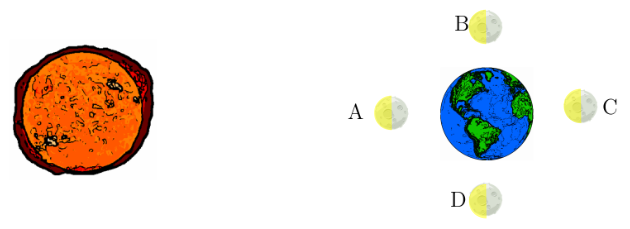
\includegraphics[width=5in]{../images/high_tides.png}
\end{center}

\textbf{A:} Someone on the Earth directly under the moon will see a new moon, since only the side directly away from the Earth is illuminated. At this point, the high tides are at their highest, since the tidal bulges caused by the Earth and moon are adding together.

\textbf{B:} Someone on the Earth directly under the moon will see half of it illuminated. Here the high tide is a little lower, because the tidal bulges caused by the Sun and Moon are perpendicular (at $90^0$) from Each other.

\textbf{C:} Someone on Earth directly under the moon will see a full moon (fully illuminated). Since the tidal bulges from the Moon and Sun are aligned, the high tide will again be at its highest point.

\textbf{D:} This is the same as for case \textit{B}.

\end{document}